\resizebox{\textwidth}{!}{%
      \centering
    \scriptsize
    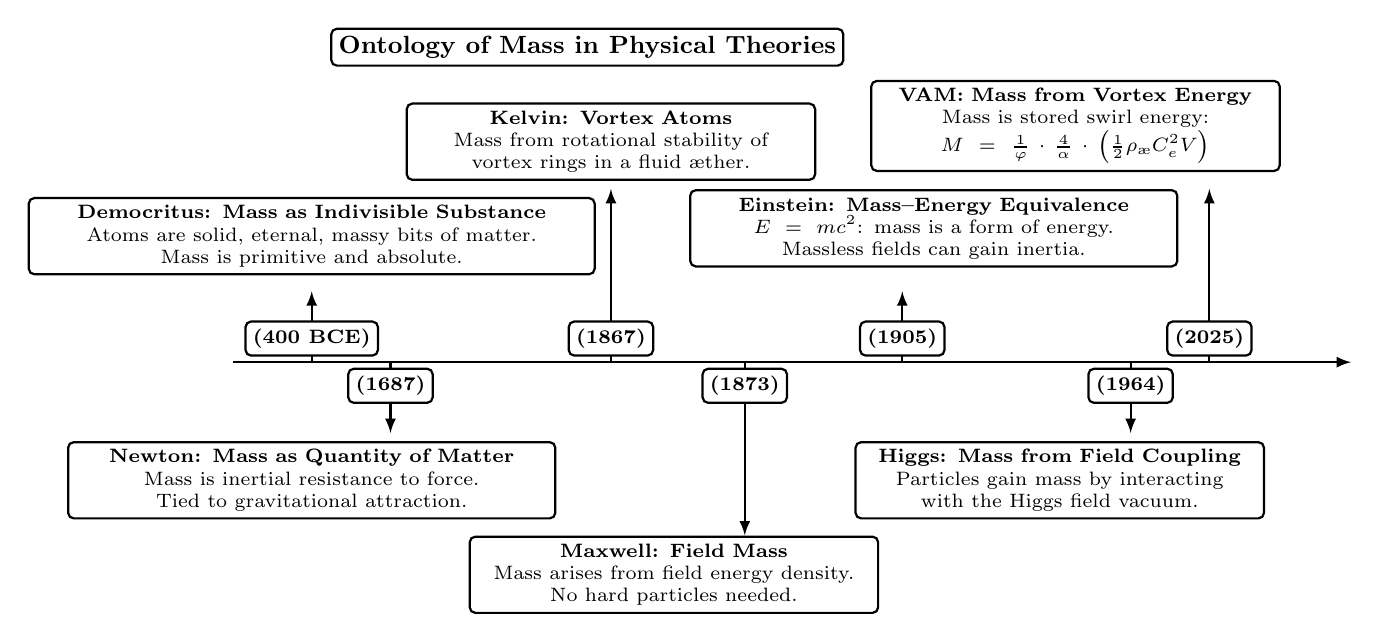
\begin{tikzpicture}[node distance=3.5cm, every node/.style={font=\scriptsize}, >=latex]
    \scriptsize

    % Timeline base
    \draw[->, thick] (-1,0) -- (13.2,0);

    % Arrows above timeline (short, as requested)
    \draw[->, thick] (0,0) -- (0,0.9);       % Pre-Socratics
    \draw[->, thick] (3.8,0) -- (3.8,2.2);   % Augustine
    \draw[->, thick] (7.5,0) -- (7.5,0.9);   % Einstein
    \draw[->, thick] (11.4,0) -- (11.4,2.2); % VAM

    % Arrows below timeline (short, as requested)
    \draw[->, thick] (1.0,0) -- (1.0,-0.9);     % Plato/Aristotle
    \draw[->, thick] (5.5,0) -- (5.5,-2.2);     % Newton
    \draw[->, thick] (10.4,0) -- (10.4,-0.9);     % Leibniz/Mach

        %--- Root title cards (above timeline) ---
    \node[draw, thick, rounded corners=2pt, fill=white, align=center, font=\bfseries ] at (0, .3)   {(400 BCE)};
    \node[draw, thick, rounded corners=2pt, fill=white, align=center, font=\bfseries ] at (3.8, .3) {(1867)};
    \node[draw, thick, rounded corners=2pt, fill=white, align=center, font=\bfseries ] at (7.5, .3) {(1905)};
    \node[draw, thick, rounded corners=2pt, fill=white, align=center, font=\bfseries ] at (11.4, .3){(2025)};

    %--- Root title cards (below timeline) ---
    \node[draw, thick, rounded corners=2pt, fill=white, align=center, font=\bfseries ] at (1.0,- .3) {(1687)};
    \node[draw, thick, rounded corners=2pt, fill=white, align=center, font=\bfseries ] at (5.5,- .3) {(1873)};
    \node[draw, thick, rounded corners=2pt, fill=white, align=center, font=\bfseries ] at (10.4,- .3) {(1964)};

    % Label
    \node[draw, thick, fill=white, rounded corners=2pt, font=\small] at (3.5,4.0) {\textbf{Ontology of Mass in Physical Theories}};

    % Democritus (left)
    \node[draw, rounded corners=2pt, thick, align=center, fill=white, text width=7cm] at (0,1.6) {
    \textbf{Democritus: Mass as Indivisible Substance}  \\% [-0.8em]
    Atoms are solid, eternal, massy bits of matter.  \\% [-0.8em]
    Mass is primitive and absolute.
    };

    % Newton (below)
    \node[draw, rounded corners=2pt, thick, align=center, fill=white, text width=6cm] at (0,-1.5) {
    \textbf{Newton: Mass as Quantity of Matter}  \\% [-0.8em]
    Mass is inertial resistance to force.  \\% [-0.8em]
    Tied to gravitational attraction.
    };


    % Kelvin (top)
    \node[draw, rounded corners=2pt, thick, align=center, fill=white, text width=5cm] at (3.8,2.8) {
    \textbf{Kelvin: Vortex Atoms}  \\% [-0.8em]
    Mass from rotational stability of  \\% [-0.8em]
    vortex rings in a fluid æther.
    };


    % Maxwell (bottom)
    \node[draw, rounded corners=2pt, thick, align=center, fill=white, text width=5cm] at (4.6,-2.7) {
    \textbf{Maxwell: Field Mass}  \\% [-0.8em]
    Mass arises from field energy density.  \\% [-0.8em]
    No hard particles needed.
    };

    % Einstein (top)
    \node[draw, rounded corners=2pt, thick, align=center, fill=white, text width=6cm] at (7.9,1.7) {
    \textbf{Einstein: Mass–Energy Equivalence}  \\% [-0.4em]
    \( E = mc^2 \): mass is a form of energy.  \\% [-0.8em]
    Massless fields can gain inertia.
    };


    % Higgs (bottom)
    \node[draw, rounded corners=2pt, thick, align=center, fill=white, text width=5cm] at (9.5,-1.5) {
    \textbf{Higgs: Mass from Field Coupling}  \\% [-0.8em]
    Particles gain mass by interacting  \\% [-0.8em]
    with the Higgs field vacuum.
    };


    % VAM (top right)
    \node[draw, rounded corners=2pt, thick, align=center, fill=white, text width=5cm] at (9.7,3.0) {
    \textbf{VAM: Mass from Vortex Energy}  \\% [-0.8em]
    Mass is stored swirl energy:  \\% [-0.4em]
    \( M = \frac{1}{\varphi} \cdot \frac{4}{\alpha} \cdot \left( \frac{1}{2} \rho_\text{\ae} C_e^2 V \right) \)
    };

    \end{tikzpicture}
    \caption{\textbf{Evolution of the concept of mass across physics:} from atomistic substance (Democritus), through Newtonian inertia and field-theoretic mass (Maxwell, Higgs), to VAM’s fluid-topological model. In VAM, mass is emergent swirl energy stored in knotted vortex configurations within a quantized æther. Each stage reflects deeper abstraction—from particles to energy to geometry to topology.}\label{fig:OntologyOfMass}
}